\subsection{Modifica LLM salvato}

\begin{figure}[H]
    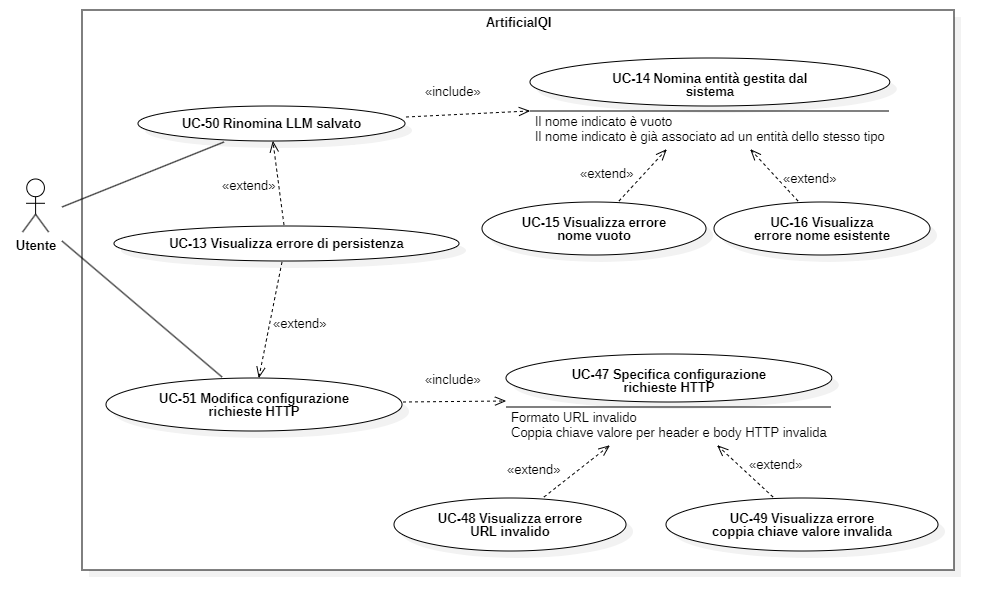
\includegraphics[scale=0.45]{Sezioni/UseCase/Immagini/ModificaLLM.png}
    \caption{Diagramma modifica LLM salvato.}
\end{figure}

\begin{usecase}{UC-50}{Rinomina LLM salvato}
    \label{uc:UC-50}
    
    \req{\hyperref[ru:RUF-6]{RUF-6}} 

    \pre{
        \item L'LLM da rinominare esiste
        \item L'utente sta visualizzando gli LLM salvati \hyperref[uc:UC-52]{UC-52}
    }

    \post{
        \item L'LLM viene rinominato
    }
    
    \actor{Utente}

    \trigger{L'utente vuole rinominare un LLM salvato}

    \inc{\hyperref[uc:UC-14]{UC-14} }

    \base{}

    \scenario{
        \item L'utente richiede la modifica dell'LLM salvato
        \item Il sistema ottiene il nuovo nome per LLM seguendo \hyperref[uc:UC-14]{UC-14}       
        \item Il sistema rinomina l'LLM
        \item Il sistema avvisa l'utente della avvenuta rinominazione
    }

    \subscenario{
        \item[3.1] Avviene un errore interno al sistema durante la rinominazione dell'LLM:
        \begin{itemize}
            \item \hyperref[uc:UC-13]{UC-13}
        \end{itemize}
    }
\end{usecase}

\begin{usecase}{UC-51}{Modifica configurazione richieste HTTP}
    \label{uc:UC-51}
    
    \req{\hyperref[ru:RUF-6]{RUF-6}} 

    \pre{
        \item L'LLM per cui si vuole modificare la configurazione esiste
        \item L'utente sta visualizzando gli LLM salvati \hyperref[uc:UC-52]{UC-52}
    }

    \post{
        \item La configurazione per l'LLM viene modificata
    }
    
    \actor{Utente}

    \trigger{L'utente vuole modificare la configurazione di un LLM salvato}

    \inc{\hyperref[uc:UC-47]{UC-47}}

    \base{}

    \scenario{
        \item L'utente richiede la modifica dell'LLM salvato
        \item Il sistema ottiene la nuova configurazione per il LLM seguendo \hyperref[uc:UC-47]{UC-47}       
        \item Il sistema aggiorna la configurazione dell'LLM
        \item Il sistema avvisa l'utente che la modifica è avvenuta con successo
    }

    \subscenario{
        \item[3.1] Avviene un errore interno al sistema durante la modifica della configurazione:
        \begin{itemize}
            \item \hyperref[uc:UC-13]{UC-13}
        \end{itemize}
    }
\end{usecase}